\section{How does an external magnetic field affect an atom in LS-coupling? Describe the Zeeman effect without accounting for the nucleus.}
\sectionmark{Zeemaneffekt for LS-kobling}

\noindent
\large
Tegn denne tegning undervejs:
\begin{itemize}
    \item 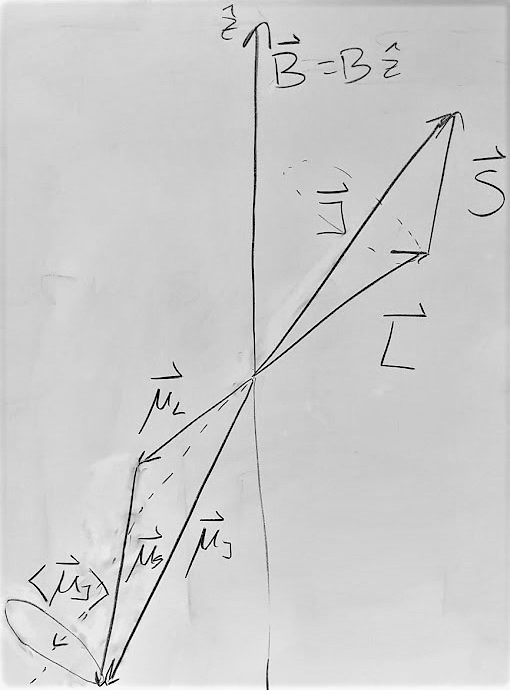
\includegraphics[width=.6\textwidth]{Q15/images/ZeemanEffectWithLSCouplingOwnDrawing.png}
\end{itemize}
%
\normalsize{Tegn højresiden af figuren, altså impulsmomenterne.}\large\\
LS-kobling
\begin{itemize}
    \item LS-koblingen er den del af finstrukturen, hvor elektronernes baneimpulsmomenter og spin kobler stærkere indbyrdes end med hinanden således, at vi kan definere det totale elektronimpulsmoment som summen af det totale baneimpulsmoment $\Vec{L}$ og det totale spin $\Vec{S}$.
\end{itemize}
%
\normalsize{Tegn venstresiden af figuren, altså dipolmomenterne.}\large\\
Dipolmomenter fra impulsmomenterne
\begin{itemize}
    \item Impulsmomenterne giver anledning til dipolmomenter, som vil være modsatrettede men parallelle med deres respektive impulsmomenter $\Vec{L}$ og $\Vec{S}$. Dermed fås det totale elektrondipolmoment
    \begin{align*}
        \Vec{\mu}_J &= -\frac{\mu_B}{\hbar}\left(g_L \Vec{L} + g_S \Vec{S}\right) \: , \quad g_L \simeq 1\: \wedge \ g_S \simeq 2 \: ,
    \end{align*}
    som grundet Landé g-faktorerne ikke vil være antiparallelt med $\Vec{J}$.
\end{itemize}
%
\normalsize{Tegn projektionen af $\Vec{\mu}_J$ på $\Vec{J}$.}\large\\
Projektion af $\Vec{\mu}_J$ på $\Vec{J}$
\begin{itemize}
    \item Idet at $\Vec{\mu}_J$ vil præcisere rundt om $\Vec{J}$-aksen, så vil de vinkelrette komponenter tidsgennemsnitligt give 0 (Larmorpræcision). Dermed projiceres $\Vec{\mu}_J$ på $\Vec{J}$
    \begin{align*}
        \braket{\Vec{\mu}_J} &= \left(\Vec{\mu}_J \cdot \Hat{J}\right) \Hat{J}
        = \left(\frac{\Vec{\mu}_J \cdot \Vec{J}}{|\Vec{J}|^2}\right) \Vec{J}
        \propto \frac{\Vec{L} \cdot \Vec{J}}{|\Vec{J}|^2} + \frac{\Vec{S} \cdot \Vec{J}}{|\Vec{J}|^2} \: .
    \end{align*}
\end{itemize}
%
\normalsize{Tegn $z$-akse og magnetfelt $\Vec{B} = B\Hat{z}$.}\large\\
Indsættes dette atom i et magnetfelt, så vil dipolmomentet vekselvirke med det magnetiske felt, hvorved vi får
\begin{align*}
    H = - \braket{\Vec{\mu}_J} \cdot \Vec{B} \propto \Vec{J} \cdot \Vec{B} = BJ_z \: .
\end{align*}\\
Energiskiftet grundet Zeemaneffekten findes ved
\begin{align*}
    E_{ZE} &= \braket{H} \propto \braket{\left(\frac{\Vec{L} \cdot \Vec{J}}{\abs{\Vec{J}}^2} + \frac{\Vec{S} \cdot \Vec{J}}{\abs{\Vec{J}}^2}\right)J_z} \: .
\end{align*}\\\\
%
Vi ved at
\begin{align*}
    \braket{\abs{\Vec{J}}^2} &= \hbar^2 J(J+1) \: , \quad \text{og} \quad \braket{J_z} = \hbar M_J \: ,
\end{align*}
og benytter definitionen af $\Vec{J}$, så (her for $\Vec{S}$, men gøres også for $\Vec{L}$)
\begin{align*}
    \Vec{S} &= \Vec{J} - \Vec{L} \Rightarrow \Vec{S}^2 = \Vec{J}^2 + \Vec{L}^2 - 2\Vec{L}\cdot\Vec{J} \: .
\end{align*}\\\\
%
Energiskiftet bliver derved
\begin{align*}
    E_{ZE} &= g_J M_J \mu_B B \: , \quad \text{hvor} \quad g_J = \frac{3}{2} + \frac{S(S+1) - L(L+1)}{2J(J+1)} \: .
\end{align*}\\\\
%
Opsplitning af tilstand med $J = 2$
\begin{itemize}
    \item 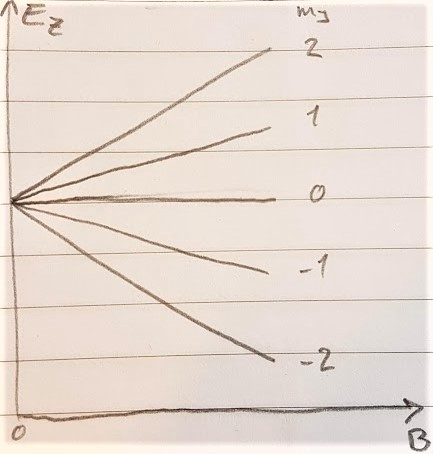
\includegraphics[width=.5\textwidth]{Q15/images/ZeemanEffectWithLSCouplingSplitting.jpg}
\end{itemize}
Normal ($S=0$) og unormal Zeemaneffekt ($S \ne 0$)
\begin{itemize}
    \item 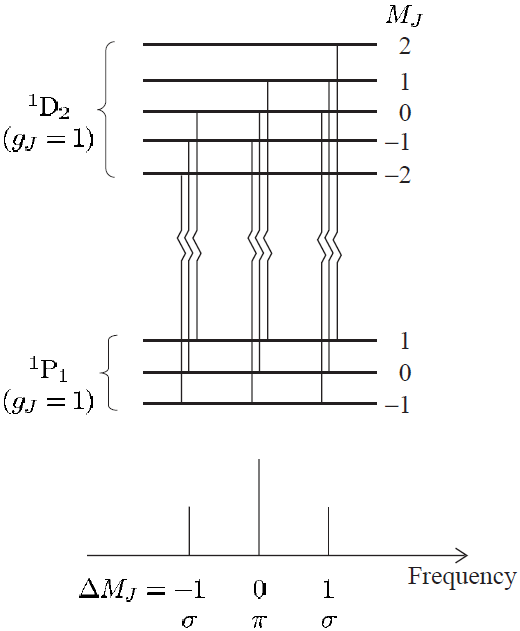
\includegraphics[width=.45\textwidth]{Q15/images/NormalZeemanEffect.PNG} \hfill 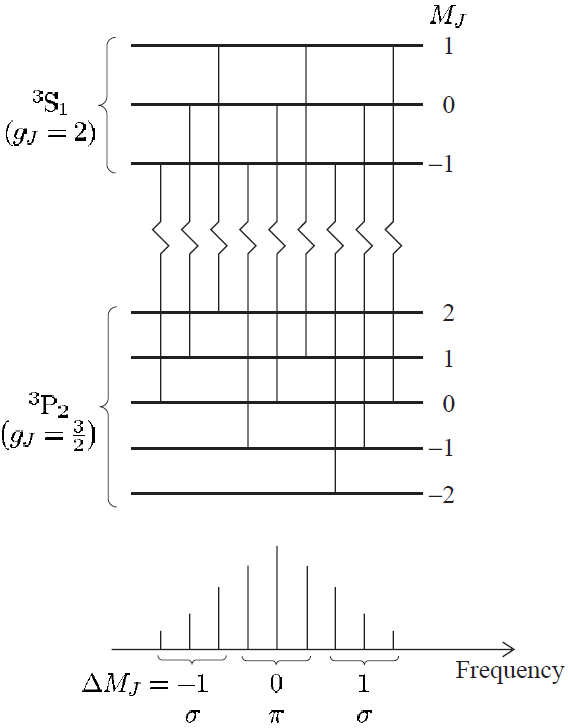
\includegraphics[width=.45\textwidth]{Q15/images/AnomalousZeemanEffect.PNG}
    \item \normalsize{Tegn kun overgangene for $\Delta M_J = -1$ for normal og udelad at tegne overgangene for unormal. Tegn kun bunden med frekvens.}\large
\end{itemize}
\normalsize